\documentclass{beamer}
\usepackage{graphicx,tabularx}
\usepackage{amsmath}

\graphicspath{ {./source/} }
\usepackage[utf8]{inputenc}

\title{Comparison of network complexity measures}
\author{Yipei Zhao}
\institute{Aston University}
\date{\today}

\begin{document}
    \frame{\titlepage}
    \begin{frame}{Network Science}
        \centering
        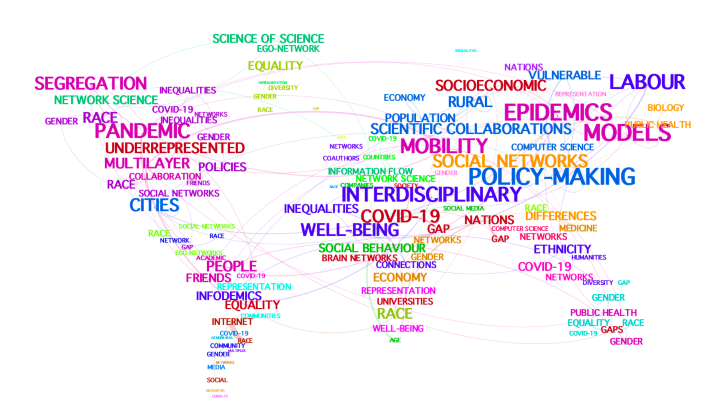
\includegraphics[width=\textwidth]{v1.png}
    \end{frame}


    \begin{frame}{Complexity measures}
        \begin{itemize}
            \item Different subgraph measures
            \begin{itemize}
                \item $C_{1e.st}$
                \item $C_{1e,spec}$
                \item $C_{2e,spec}$
            \end{itemize}
            \item Product measures
            \begin{itemize}
                \item $MA_g$
                \item $MA_{RI}$
                \item $Cr$
                \item $Ce$
            \end{itemize}
            \item Entropy measure
            \begin{itemize}
                \item $OdC$
            \end{itemize}
        \end{itemize}
    \end{frame}


    \begin{frame}{$MA_{RI}$}
        A product measure that is based on the idea of $MA_g$.
        \begin{itemize}
            \item Redundancy of a graph: $R=\frac{1}{m}\sum_{i,j>i}ln(d_id_j)$
            \item Mutual information of a graph: $I=\frac{1}{m}\sum_{i,j>i}ln(\frac{2m}{d_id_j})$
            \item Highest redundancy: $R_{clique} = 2ln(n-1)$
            \item Lowest redundancy: $R_{path} = 2(\frac{n-2}{n-1})ln(2)$
            \item Highest mutual information: $I_{path} = ln(n-1)-(\frac{n-3}{n-1})ln2$
            \item Lowest mutual information: $I_{clique}=ln(\frac{n}{n-1})$
            \item $C = (R - R_{path})(I-I_{clique})$
        \end{itemize}
    \end{frame}


    \frame{Result}
    \frame{Conclusion}


    \begin{frame}{Reference}
        \begin{enumerate}
            \item {\url https://appliednetsci.springeropen.com/networked-inequality--studies-on-diversity-and-marginalization}
        \end{enumerate}        
    \end{frame}
\end{document}